\documentclass[crop,tikz,border=10px,convert=pdf2svg,multi=false]{standalone}
\usepackage{amsfonts}
\usepackage[defaultsans]{opensans}
\usetikzlibrary{shapes,arrows,positioning}
\begin{document}
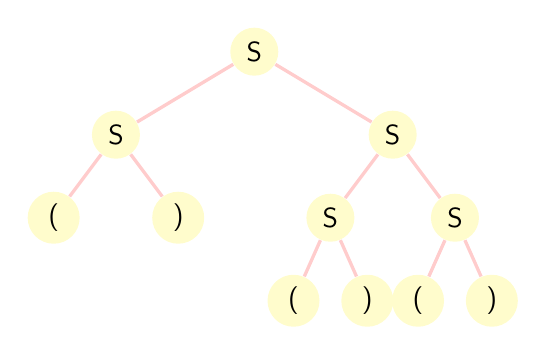
\begin{tikzpicture}[font=\sffamily,level distance=3em,
  treenode/.style = {circle, fill=yellow!20, align=center, inner
    sep=.3em, text centered},
  level/.style={sibling distance=11em/#1-1em},
  edge from parent/.style={red!20,very thick,draw}]

  \node [treenode] (root) {S}
  child {
    node [treenode] {S}
    child {node [treenode] {(}}
    child {node [treenode] {)}}
  }
  child {
    node [treenode] {S}
    child {
      node [treenode] {S}
      child {node [treenode] {(}}
      child {node [treenode] {)}}
    }
    child {
      node [treenode] {S}
      child {node [treenode] {(}}
      child {node [treenode] {)}}
    }
  };

\end{tikzpicture}
\end{document}
